\documentclass[10pt, t]{beamer}
% \usepackage[UTF8]{ctex}
\usepackage{amsmath}
\usepackage{setspace}
\usepackage{float} 
\usepackage{multido}
\usepackage{multirow}
\usepackage{array}
\usepackage{enumerate}
\usepackage{booktabs}
\usepackage{indentfirst} 
\usepackage[style=mla]{biblatex}
\usepackage{setspace}
\usepackage{subcaption}
\usepackage{hyperref}
\usepackage{textpos}
% \usepackage{fontspec}

\makeatletter
\let\@@magyar@captionfix\relax
\makeatother

\definecolor{bladerunnerblue}{RGB}{41, 159, 163}
\definecolor{bladerunnerred}{RGB}{194,84,97}
\definecolor{themecolor}{RGB}{25,25,112} 
\definecolor{weak}{RGB}{150,150,150}

\renewcommand{\emph}[1]{{\color{themecolor}\textsl{#1}}}
\newcommand{\alarm}[1]{{\color{bladerunnerred}{#1}}}
\newcommand{\N}{\mathbb{N}}
\newcommand{\R}{\mathbb{R}}
\newcommand{\myseries}[2]{$#1_1,#1_2,\dots,#1_#2$}
\newcommand{\nullspace}{~\\[15pt]}
\newcommand{\remark}{\textbf{Remark: }}
\newcommand{\scp}[2]{\langle\,#1\,,\,#2\,\rangle} \newcommand{\scpp}{\langle\,\cdot\,,\,\cdot\,\rangle}
\newcommand{\weaken}[1]{{\color{weak}\textit{#1}}}
\newcommand{\underover}[3]{\underset{#2}{\overset{#3}{#1}}}
\renewcommand{\emptyset}{\varnothing}


\usetheme{Madrid}
\setbeamertemplate{navigation symbols}{}

\addtobeamertemplate{frametitle}{}{
\begin{textblock*}{100mm}(0.85\textwidth,-1cm)
\includegraphics[height=1cm]{../../logo.png}
\end{textblock*}}


\usecolortheme[named=themecolor]{structure}

\setbeamertemplate{items}[default]

\hypersetup{
    colorlinks=true,
    linkcolor=themecolor,
    filecolor=themecolor,      
    urlcolor=themecolor,
    citecolor=themecolor,
}

\title{VV186: Honors Mathematics}
\subtitle{\large Math Foundations}
\institute[UM-SJTU JI]{Univerity of Michigan-Shanghai Jiao Tong University Joint Institute}
\author{Xingjian Zhang}

\begin{document}

\begin{frame}
    \titlepage
    \begin{center}
        \includegraphics[height=2cm]{../../logo2.png}
    \end{center}
\end{frame}

\begin{frame}
    \frametitle{Pay attention to...}
    Several things I want you to pay attention to:
    \begin{enumerate}
        \item \alarm{Be interactive.} Feel free to interrupt me at any time if you want to ask something or simply make some comments. You are free to discuss with your friend if you want, as long as your discussion is related to the course contents and your voice won't effect other students.
        \item Speak everything in \alarm{English} during the RC. This might be hard at the beginning, but you will soon get used to that.
        \item \alarm{``Question everything.''} Do not pretend to have understood everything. Maths is about strictness, abstraction and generalization. Understanding every basic concept is essential in our course. I will be quite ``push'' on checking your conceptual understanding. This process will be \textbf{annoying, tedious, but rewarding}. So Get prepared.
        \item \alarm{Open the camera if you can.} This is important for me. It is hard to keep talking for more than one hour without seeing any feedback from you. Convince yourself that your small action does make my life easier. So please open your camera.
    \end{enumerate}
\end{frame}

\begin{frame}
    \frametitle{Outline}
    \begin{spacing}{1}
        \tableofcontents
    \end{spacing}
\end{frame}

\section{Natural Number and Mathematical Induction}
\begin{frame}
    \frametitle{Natural Number}
    What is the seven properties of natural numbers' operations?\nullspace
    \pause
    \begin{enumerate}
        \item
              associativity$\times 2$
        \item
              existence of neutral element$\times 2$
        \item commutativity$\times 2$
        \item distributivity.
    \end{enumerate}
\end{frame}

\begin{frame}
    \frametitle{Notation for Addition \& Multiplication}
    \begin{figure}[H]
        \centering
        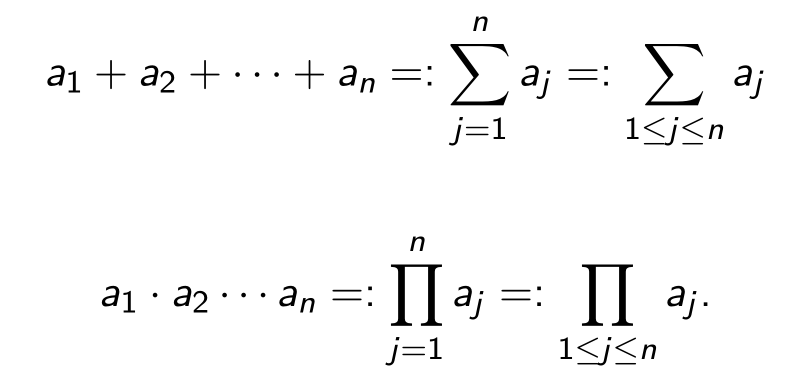
\includegraphics[width=0.5\textwidth]{2020-09-23-13-08-15.png}
    \end{figure}
\end{frame}

\begin{frame}
    \frametitle{Mathematical Induction}

    \begin{figure}[H]
        \centering
        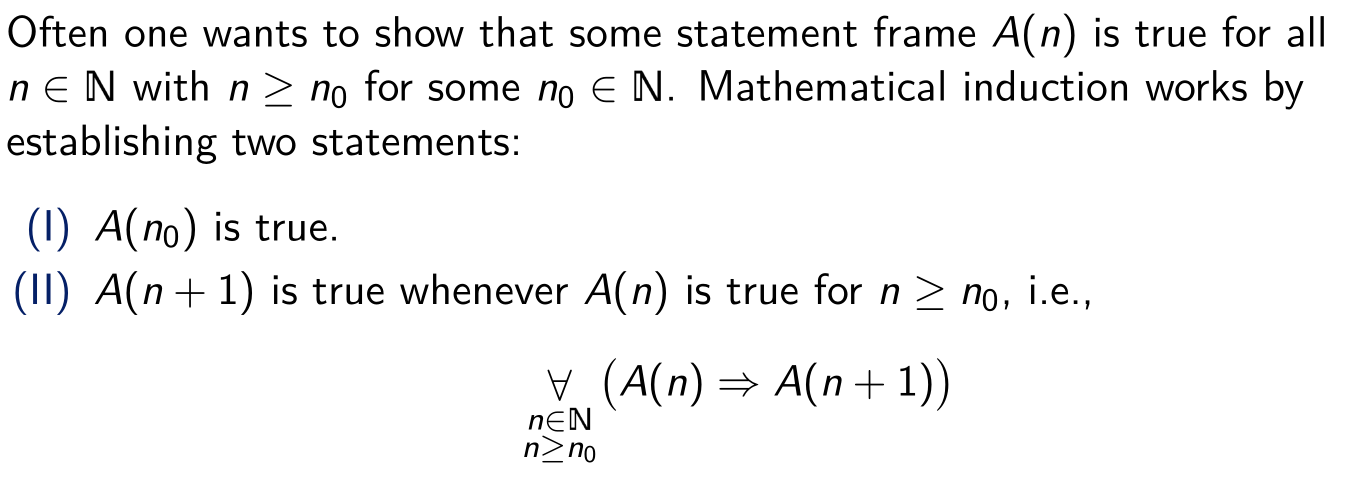
\includegraphics[width=0.9\textwidth]{2020-09-23-12-37-23.png}
    \end{figure}
    Straightforward Exercise:\nullspace Prove
    \begin{center}
        For all $n\in \N$, $5^n - 1$ is divisible by 4.
    \end{center}
\end{frame}

\begin{frame}[allowframebreaks]
    \frametitle{Conceptually Interesting Exercise}

    Let's see an interesting problem. What is going wrong in the proof?
    \begin{figure}[H]
        \centering
        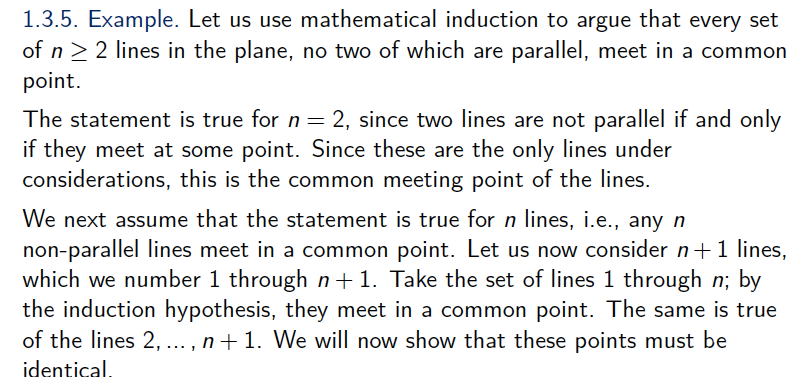
\includegraphics[width=0.9\textwidth]{2020-09-23-13-12-35.png}
    \end{figure}
    \begin{figure}[H]
        \centering
        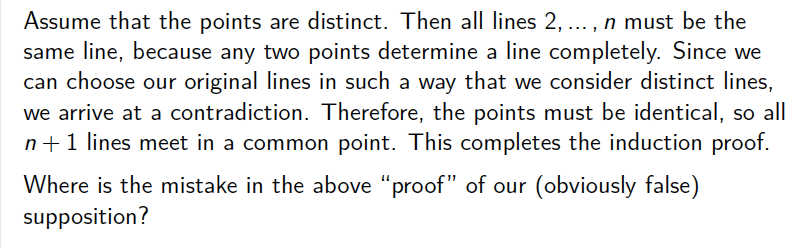
\includegraphics[width=0.9\textwidth]{2020-09-23-13-13-41.png}
    \end{figure}
    \textbf{Hint:} Start by considering the case where $n=3$, find some contradiction to invalidate the above proof.\nullspace
    \textbf{Remark:} Induction can sometimes be tricky. Before using it, examine the complex level of the problem, because using induction is sometimes
    much more complicated than using a ``direct'' method to prove a statement.
\end{frame}

\section{Rational Number}
\begin{frame}
    \frametitle{Rational Number}
    $$\mathbb{Q}=\left\{\frac{p}{q}: p, q \in \mathbb{Z} \wedge q \neq 0\right\}$$
    What is the 12 properties of $\mathbb{Q}$?
    \pause
    \begin{itemize}
        \item $\mathbb{Q}$ inherits all the 7 properties of $\N$
        \item inverse element of $+$ and $\cdot$
        \item trichotomy law
        \item closed under $+$ and $\cdot$
    \end{itemize}
    \nullspace
    \textbf{Simple Exercise:}
    With these properties, prove
    \begin{enumerate}
        \item
              if $a\neq 0$ and $a \cdot b = a \cdot c$, then
              $b = c$.
        \item
              Furthermore,if $a \cdot b = 0$, then either$ a = 0 $ or $ b = 0$.
        \item  $a - b = b - a$ only if $a = b$
    \end{enumerate}
\end{frame}

\begin{frame}
    \frametitle{Triangle Inequality}

    For all rational numbers $a,b\in Q$, we have
    $$|a + b| \leq |a| + |b|.$$ Furthermore,
    $$|a + b| \geq    \left||a| - |b|\right| $$
    \nullspace
    \textbf{Remark:} They are quite useful in proof. We will see example(s) later.
\end{frame}

\begin{frame}
    \frametitle{Boundness}

    How do we define these concepts?
    \begin{enumerate}
        \item bounded/unbounded
        \item $\max,\min$
        \item $\sup,\inf$
    \end{enumerate}
    What's the relationship between 1. and 2.? (how to prove?) Does a set in $\mathbb{Q}/\R$ necessarily has a $\max$ or $\sup$?
\end{frame}

\begin{frame}
    \frametitle{Classification of Points}
    Let $A\in \R$ be any set.
    \begin{enumerate}
        \item
              We call $x \in \mathbb{R}$ an \emph{interior point} of $A$ if there exists some $\varepsilon>0$ such that the interval $(x-\varepsilon, x+\varepsilon) \subset A .$ The set of interior points of $A$ is denoted by int $A$.
        \item
              We call $x \in \mathbb{R}$ an \emph{exterior point} of $A$ if there exists some $\varepsilon>0$ such that the interval $(x-\varepsilon, x+\varepsilon) \cap A=\emptyset$
        \item
              We call $x \in \mathbb{R}$ a \emph{boundary point} of $A$ if for every $\varepsilon>0$ $(x-\varepsilon, x+\varepsilon) \cap A \neq \emptyset$ and $(x-\varepsilon, x+\varepsilon) \cap A^{c} \neq \emptyset .$ The set of boundary points of $A$ is denoted by $\partial A$.
        \item
              We call $x \in \mathbb{R}$ an \emph{accumulation point} of $A$ if for every $\varepsilon>0$ the interval $(x-\varepsilon, x+\varepsilon) \cap A \backslash\{x\} \neq \emptyset$
    \end{enumerate}
    \textbf{Remark:} We will discuss more on sets and classification of points in $\R^n$ in VV285.

\end{frame}

\section{Complex Numbers}
\begin{frame}
    \frametitle{Complex Numbers}
    We define \emph{complex numbers} in order to resolve the algebraic incompleteness of real numbers. The formal definition makes use of the ordered pairs, so that $\R^2\cong\mathbb{C}$. But in practice, we usually use the notation $a+bi$ rather than $(a,b)$ to indicate a complex number $z$.\nullspace
    We define the modulus or absolute value of a complex number $z=a+b i$ by
    $$
        |z|=\sqrt{a^{2}+b^{2}}=\sqrt{z \cdot \bar{z}}
    $$
    Here $\bar{z}=a-b i$ is called the complex conjugate of $z$\nullspace
    Let $z_{0} \in \mathbb{C} .$ Then we define the open ball of radius $R>0$ centered at $z_{0}$ by
    $$
        B_{R}\left(z_{0}\right):=\left\{z \in \mathbb{C}:\left|z-z_{0}\right|<R\right\}
    $$
    \textbf{Remark:} * We will generalize the concept of open ball to $\R^n$ or $\mathbb{C}^n$ in VV285. Additionally, complex analysis is an important topic of VV286, which turns out to be extremely useful in several fields: Fourier Analysis, Improper Integral, and Ordinary Differential Equations.
\end{frame}

\section{Functions}
\begin{frame}
    \frametitle{Functions}
    We use a \textit{static} method to define the functions formally. To be more precise, we use predicates and sets:
    \begin{figure}[H]
        \centering
        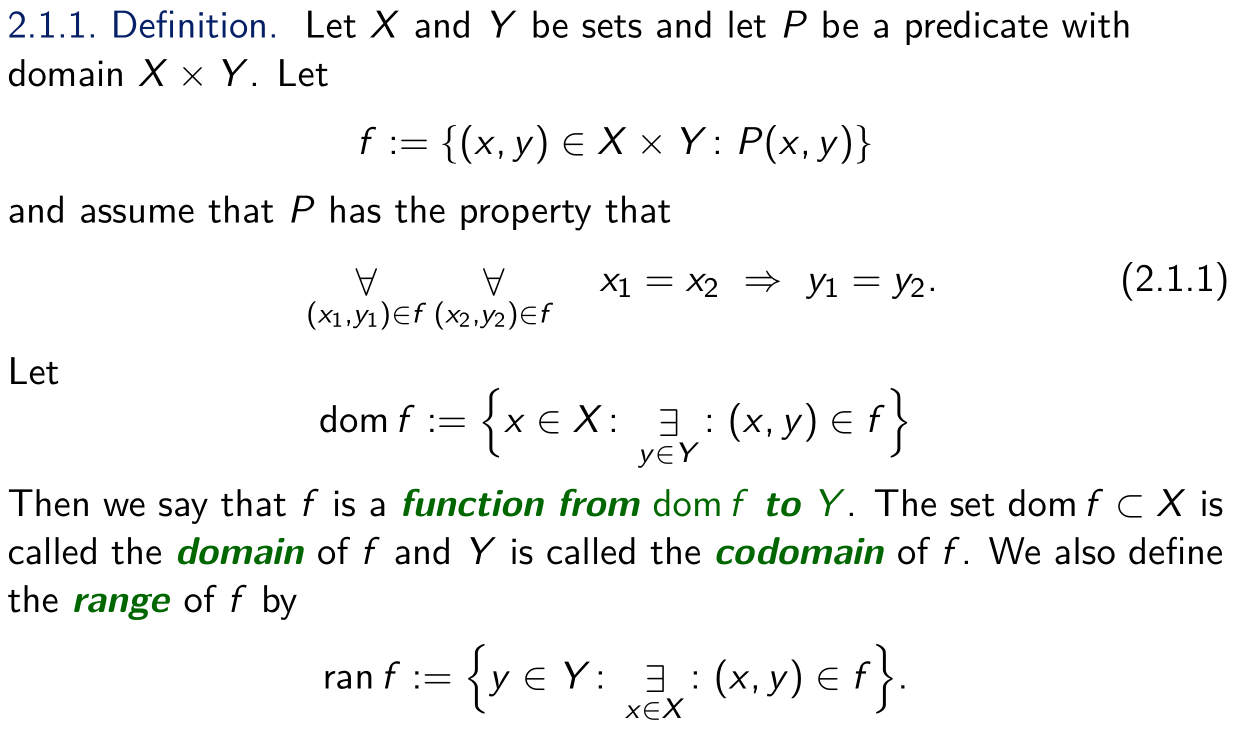
\includegraphics[width=0.9\textwidth]{2020-09-30-12-16-15.png}
    \end{figure}
\end{frame}

\begin{frame}
    \frametitle{Clarification}

    \begin{itemize}
        \item[$\times$] Co-domain of $f$ = $\operatorname{ran} f$ (Counter-example: $f:\R\to\R,x\mapsto x^2.$)
        \item[$\surd $] Domain of $f$ contains exactly all the elements that
              have assignment with an element in $f$’s co-domain.
    \end{itemize}

\end{frame}

\begin{frame}
    \frametitle{Notation of Function}

    Notation of functions is important because you will see them frequently in the coursework, and you are going to declare functions in the same way.
    $$f:\Omega\to Y,\qquad x\mapsto f(x)$$
    * Notice that the two arrows are different. The first is called ``$\backslash$to''  while the second is called ``$\backslash$mapsto'' in \LaTeX.

\end{frame}

\begin{frame}
    \frametitle{Composition of Functions}
    \begin{figure}[H]
        \centering
        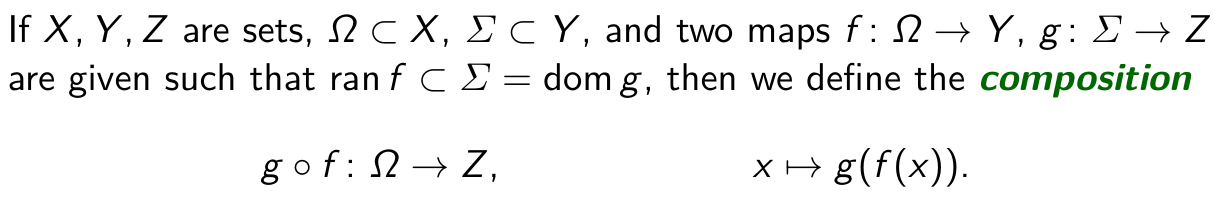
\includegraphics[width=\textwidth]{2020-09-30-13-34-51.png}
    \end{figure}

\end{frame}

\section{Sequence}
\begin{frame}
    \frametitle{Sequence}

    A sequence is essentially a map (function) from subset of $\N$ to $\R$ or $\mathbb{C}$. We allow three notations for sequence:
    $$\left(a_{n}\right)_{n \in \Omega}=\left(a_{n}\right)=a_{0}, a_{1}, a_{2}, \ldots$$
    Notice that  $(a_n)$ denotes a sequence while $a_n$, the n$^th$ term in the sequence, is a value/number.
    \nullspace\textbf{Remark:} Roughly speaking, we can define a sequence in two ways:
    \begin{itemize}
        \item Explicit definition. e.g. $(a_n)=(2n)$
        \item Recursive definition. e.g. $a_0=0, a_n=a_{n-1}+2$.
    \end{itemize}
    In general, explicit definition contains more information than a recursive definition. For example, if we know the explicit definition of \emph{Fibonacci sequence}, we can calculate its 1000$^{th}$ term in a very short time without recourse to a recursive calculation.\footnote[frame]{*$F_{n}=\frac{\varphi^{n}-\psi^{n}}{\varphi-\psi}=\frac{\varphi^{n}-\psi^{n}}{\sqrt{5}}$ where $\varphi=\frac{1+\sqrt{5}}{2}$ and $\psi=\frac{1-\sqrt{5}}{2}=1-\varphi=-\frac{1}{\varphi}$.} Finding the explicit definition of a sequence given its recursive definition is an important topic in \emph{VE203: Discrete Mathematics}.
\end{frame}

\begin{frame}[allowframebreaks]
    \frametitle{Convergence of Sequence}
    The definition of convergence (of sequence) is very important. Memorize it!
    \newpage
    \begin{figure}[H]
        \centering
        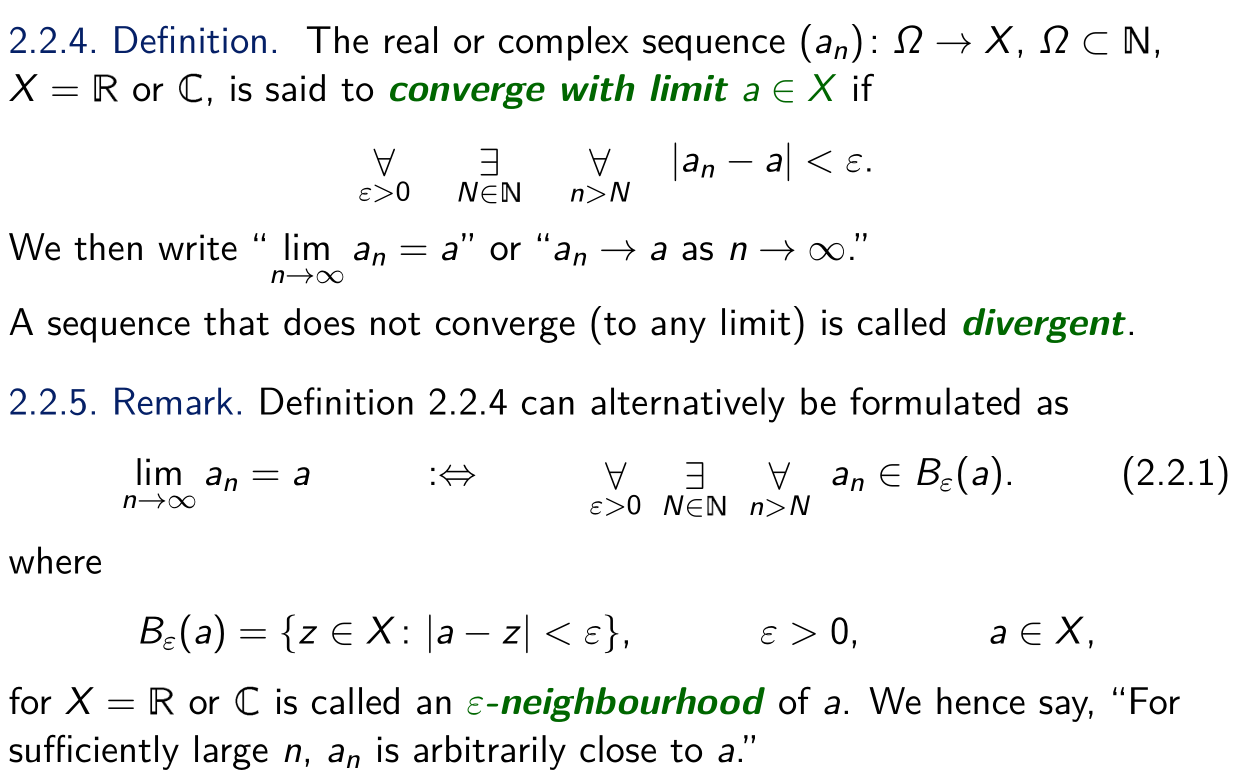
\includegraphics[width=0.8\textwidth]{2020-09-30-13-54-19.png}
    \end{figure}
    \newpage
    \begin{figure}[H]
        \centering
        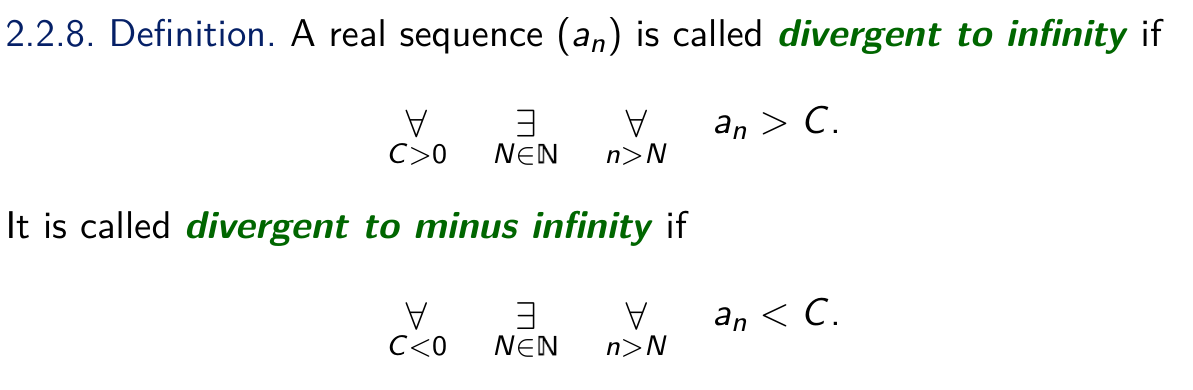
\includegraphics[width=0.9\textwidth]{2020-09-30-14-14-20.png}
    \end{figure}
    \begin{figure}[H]
        \centering
        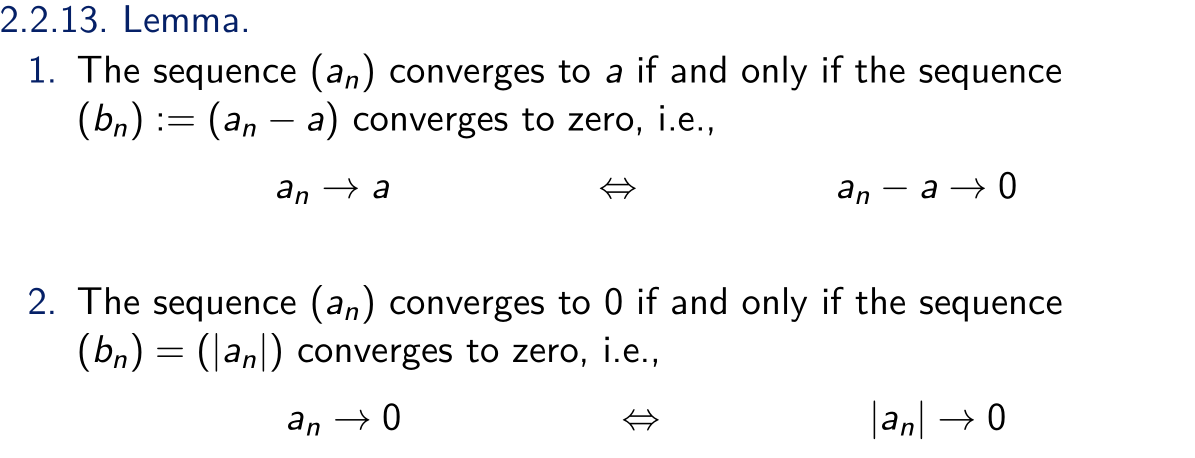
\includegraphics[width=0.9\textwidth]{2020-09-30-14-19-17.png}
    \end{figure}
    \textbf{Remark:} The above conclusion is useful in proof.
\end{frame}

\begin{frame}
    \frametitle{Clarification}

    \begin{itemize}
        \item[$\times$] A sequence may not contain infinitely many terms.\\
              When we say “sequence” we usually assume that it is infinite. If it is
              finite in number of terms, we usually say it is a ``tuple''. Similarly, a subsequence of a sequence is infinite in size, too.
        \item[$\times$] A sequence is either convergent or divergent to infinity. (Counter-example: $(a_n)=(-1)^n$)\\
              iI a sequence is not convergent, we say it is “divergent”.
              However, it doesn’t mean it diverge to $\infty$.
    \end{itemize}
\end{frame}

\begin{frame}
    \frametitle{Exercise}
    Let $(a_n)$ be a real sequence that converges to some element $L\in\R$. Prove that the sequence $\left( \dfrac{\Sigma_{i=1}^na_i}{n}\right)$ is convergent to $L$.
    \pause
    \nullspace How do we solve this kind of problem? (use the definition of convergence)
    \begin{enumerate}
        \item Fix $\varepsilon$
        \item Find $N\in\N$, so that $\forall n>N:\dots$
    \end{enumerate}

\end{frame}

\begin{frame}
    \frametitle{Solution}

    

\end{frame}

\begin{frame}
    \frametitle{Describe a Sequence}

    \begin{figure}[H]
        \centering
        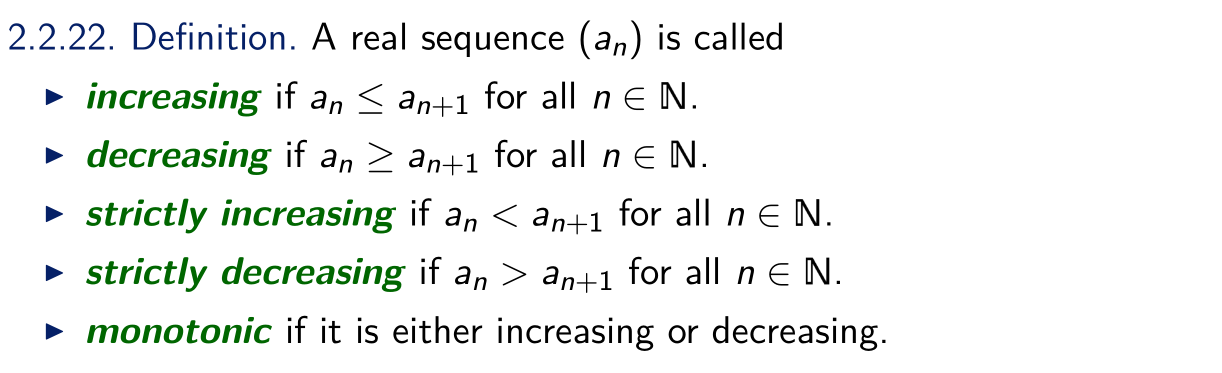
\includegraphics[width=0.9\textwidth]{2020-09-30-14-42-44.png}
    \end{figure}

\end{frame}

\begin{frame}
    \frametitle{Lemmas \& Theorems}
    \begin{enumerate}
        \item A convergent sequence is bounded.
        \item A convergent sequence has precisely one limit.
        \item \emph{Squeeze theorem.}
        \item Every monotonic and bounded (real) sequence is convergent.
        \item Let $(a_n)$ be a convergent sequence with limit $a$. Then any
              subsequence of $(a_n)$ is convergent with the same limit.
        \item Every real sequence has a monotonic subsequence.
        \item  A number a is an accumulation point of a sequence $(a_n)$
              if and only if there exists a subsequence of $(a_n)$ that converges to $a$.
        \item \emph{Theorem of Bolzano-Weierstraß.} Every bounded real sequence has
              an accumulation point.
    \end{enumerate}
    \textbf{Remark:} The squeeze theorem is useful in finding the limit of a sequence. (Try to use it to prove $\lim \sqrt[n]{n}=1$.) The Theorem of  Bolzano-Weierstraß turns out to be useful in proving the metric space $(\R, \rho)$ is complete where $\rho$ is the normal Euclidean metric in $\R$. We will further generalize this theorem in VV285, where we consider more general sequence (sequence of vector).
\end{frame}

\begin{frame}[allowframebreaks]
    \frametitle{Results of Limit Operations}
    Let $\left(a_{n}\right)$ and $\left(b_{n}\right)$ be convergent real or complex sequences with $a_{n} \rightarrow a$ and $b_{n} \rightarrow b$ for some $a, b \in \mathbb{C}$. Then
    \begin{enumerate}[(1)]
        \item 
        $\lim \left(a_{n}+b_{n}\right)=a+b$
        \item
        $\lim \left(a_{n} \cdot b_{n}\right)=a b$
        \item
        $\lim \frac{a_{n}}{b_{n}}=a / b$ if $b \neq 0$
    \end{enumerate}
    \textbf{Proof of (3):} \\
    {\footnotesize
    We want to prove that $\left|\frac{a_n}{b_n}-\frac{a}{b} \right|\rightarrow 0$ as $n\rightarrow \infty$. We can first fix some $M\in\N$ such that $\forall n>M:|b_n-b|<|b|/2$. Now, we have $\forall n>M$,
    $$\left|\frac{a_{n}}{b_{n}}-\frac{a}{b}\right|=\left|\frac{a_{n} b-b_{n} a}{b_{n} b}\right|=\left|\frac{a_{n} b-a b+a b-b_{n} a}{b_{n} b}\right| $$ 
    $$\leq \frac{\left|a_{n}-a\right||b|}{\left|b_{n} b\right|}+\frac{|a|\left|b-b_{n}\right|}{\left|b_{n} b\right|}<\frac{2\left|a_{n}-a\right||b|}{b^{2}}+\frac{2|a|\left|b-b_{n}\right|}{b^{2}}$$
    
    Given $\varepsilon>0$, choose $N>M$ such that $\forall n>N: |a_n-a|<\frac{|b|\varepsilon}{4},|b-b_n|<\frac{b^2\varepsilon}{4|a|}$. Eventually we have
    $$
        \forall \varepsilon>0\quad \exists N\in \N\quad \forall n>N:\left|\frac{a_{n}}{b_{n}}-\frac{a}{b}\right|<\frac{|b| \varepsilon}{4} \cdot \frac{2|b|}{b^{2}}+\frac{2|a|}{b^{2}} \cdot \frac{b^{2}}{|a|} \cdot \frac{\varepsilon}{4}<\varepsilon
    $$}
    \newpage
    \textbf{Extension:} Here are some other results:
    \begin{enumerate}[(1)]
        \item $\lim \sqrt{a_n}=\sqrt{\lim a_n}$ if $a_n>0$
        \item $\lim a_n^2=(\lim a_n)^2$
        \item $\lim \sqrt[n]{n}=1$
        \item $\dots$
    \end{enumerate}
    \textbf{Remark:} (1) and (2) hold for higher power, too.
\end{frame}

\begin{frame}
    \frametitle{Exercise}

    Let's see a conceptually interesting exercise: \nullspace
    Let $(p_n)_{n\in\N}$ be a sequence, and 
    $$p_0=1, p_n=\sqrt{2 p_{n-1}}$$
    Please find its limit, if exists.\nullspace
    \pause
    What do we need to do?
    \begin{enumerate}
        \item Write down the first several terms on the draft paper, and see if there's some clues. (Result: We guess that the limit exists.)
        \item Prove the existence of the limit. (How?)
        \item Calculate the limit. (How?)
    \end{enumerate}
\end{frame}

\begin{frame}
    \frametitle{Solution}

    

\end{frame}

\begin{frame}
    \frametitle{Summary}
    \textbf{About Course Contents:}\\
    As you can see, \textbf{sequence} is a very important concept in the first part of VV186. So I encourage you to review the definitions, lemmas, and theorems of them carefully before the exam. In particular, proof in the slides are valuable, because it does not only validate every theorem but also show a strict logic that you need to follow in the coursework. \nullspace
    \textbf{About Assignment:}\\
    On the one hand, you might feel Assignment 2 is much harder than Assignment 1. On the other hand, it becomes more and more exciting and interesting. Always try your best to finish the assignments independently, this will greatly helps you prepare the exams. Please feel free to ask questions on the Piazza, including questions regarding assignments. And, feel free to come to TA's OH and have some chat with us. We are glad to help you.
\end{frame}



\begin{frame}
    \frametitle{End}
    \vspace{2.2cm}
    \begin{center}
        \Large
        Have Fun \\
        And \\
        Learn Well!\footnote[frame]{Special acknowledgement to former TA Zhang Leyang, who offered many exercises and advice to my recitation class.}
    \end{center}
\end{frame}

\end{document}